\title{Bras mécanique et sudoku}
\author{Laurent Tainturier \& Alphonse TERRIER}
\date{2016-2017}
\documentclass[12pt,a4paper]{report}
\usepackage[utf8]{inputenc}
\usepackage[T1]{fontenc}
\usepackage[francais]{babel}
\usepackage{hyperref}
\usepackage{lmodern}
\usepackage{graphicx}
\usepackage{listings}
\usepackage{enumitem}
\usepackage{stmaryrd}
\usepackage{array}
\usepackage{minted}
\usepackage{color}
\usepackage{float}
\usepackage[backend=biber, autolang=other, sorting=none, style=science]{biblatex}
\usepackage[left=4cm,right=3cm,top=2.5cm,bottom=2.5cm]{geometry}
\usepackage{fancyvrb}
\frenchbsetup{StandardLists=true}
\newtheorem{theo}{Définition}[section]
\definecolor{lightgray}{gray}{.6}
\usepackage[dvipsnames]{xcolor}
\definecolor{yellow}{RGB}{225,220,0}

\newenvironment{changemargin}[2]{\begin{list}{}{%
\setlength{\topsep}{0pt}%
\setlength{\leftmargin}{0pt}%
\setlength{\rightmargin}{0pt}%
\setlength{\listparindent}{\parindent}%
\setlength{\itemindent}{\parindent}%
\setlength{\parsep}{0pt plus 1pt}%
\addtolength{\leftmargin}{#1}%
\addtolength{\rightmargin}{#2}%
}\item }{\end{list}}

\usepackage{placeins}



%\addbibresource{bibli.bib}

\begin{document}
\FloatBarrier

\begin{titlepage}
\begin{changemargin}{-1cm}{0cm}
	\centering
	\vspace{5cm}
	{\scshape\huge Institut Supérieur d'Électronique de Paris \par}
	\vspace{1cm}
	{\scshape\LARGE TIPE\par}
	\vspace{1.5cm}
	{\fontsize{45}{45}\selectfont\bfseries Bras mécanique et sudoku\par}
	\vspace{2cm}
	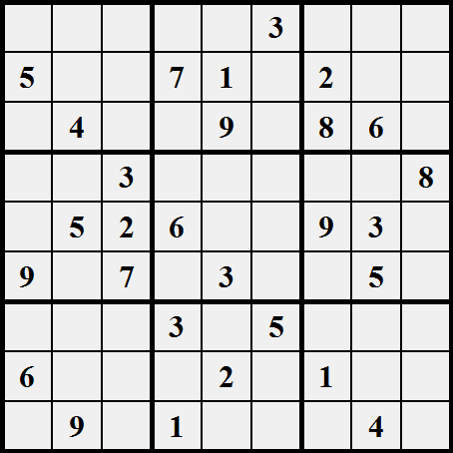
\includegraphics[width=0.7\textwidth]{../pictures/pagedegarde.png}\par\vspace{1.5cm}
	{\LARGE Laurent Tainturier \& Alphonse Terrier\par}
	\vfill
	\large supervisé par\par
	\large \bfseries M. Patrick COUVEZ

	\vfill


	{\large 2016-2017}
\end{changemargin}
\end{titlepage}

\tableofcontents
\addcontentsline{toc}{chapter}{Introduction}
\chapter*{Introduction}
	

	\chapter{Présentation du sudoku}
	
	\chapter{Électronique}
	\chapter{Mécanique}
	\chapter{Informatique}
	Tous les algorithmes sont implémentés en Python. Ils sont disponibles en annexe.
	\section{Reconnaissance du sudoku}
	Le script de reconnaissance du sudoku a été réalisé sous Python 2 avec le module de traitements d'image OpenCV. Il a été réalisé pour :
	\begin{enumerate}
	\item Reconnaître les chiffres dans une grille du sudoku
	\item Déterminer la position spatiale de la grille
	\end{enumerate}
	On photographie la grille avec une caméra Raspberry Pi (V2) comme celle-ci :
	\begin{figure}[!h]
 \center
 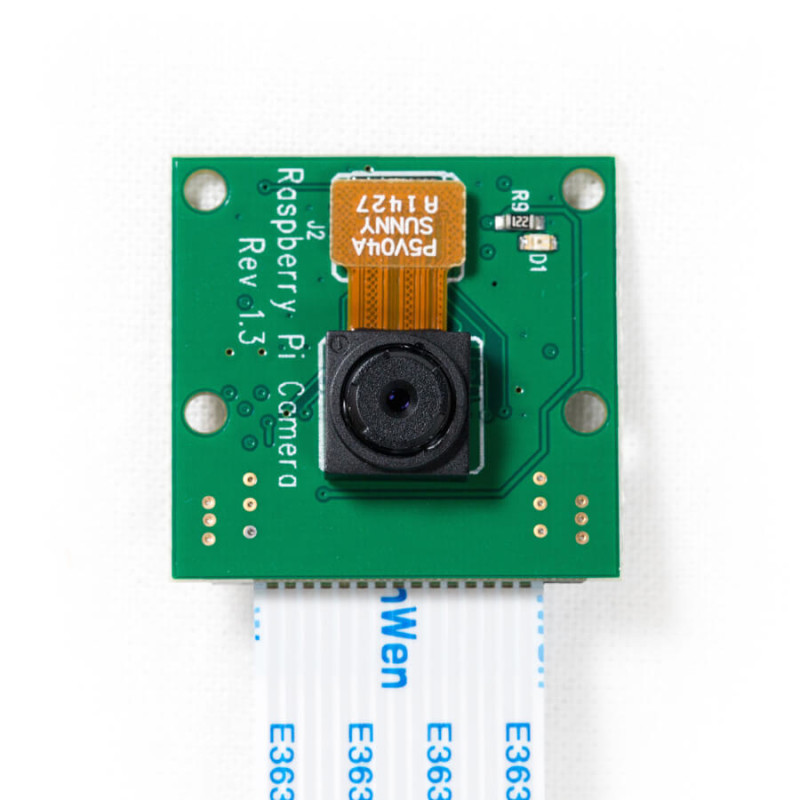
\includegraphics[scale=0.2]{../pictures/camera.jpg}
 \caption{Caméra Raspberry Pi V2}
\end{figure}
\newpage
Voici la grille de sudoku qui nous servira d'exemple pour montrer toutes les actions du script :
\begin{figure}[!h]
 \center
 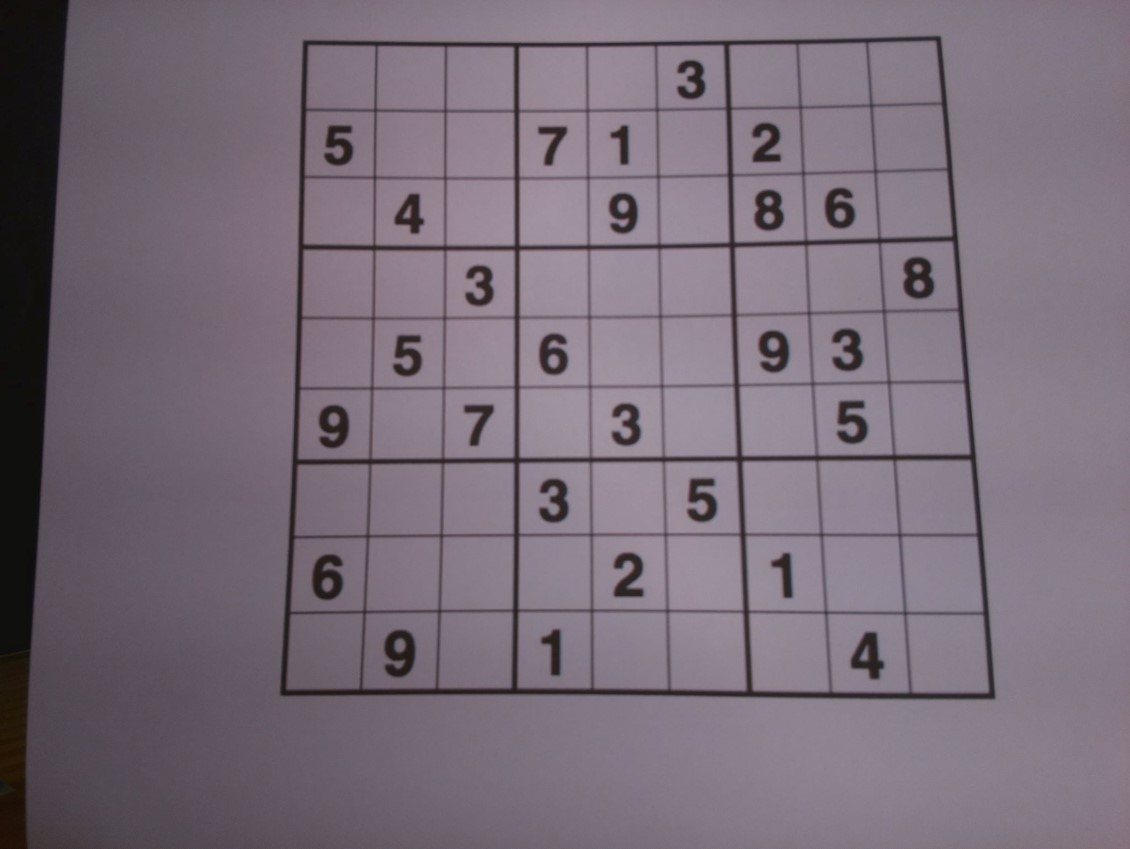
\includegraphics[scale=0.2]{../pictures/example.jpg}
 \caption{Exemple de grille de sudoku}
\end{figure}

On applique sur cette photographie un filtre de type seuil (en anglais "threshold") qui va ensuite nous permettre de détecter les contours de la grille :

\begin{figure}[!h]
 \center
 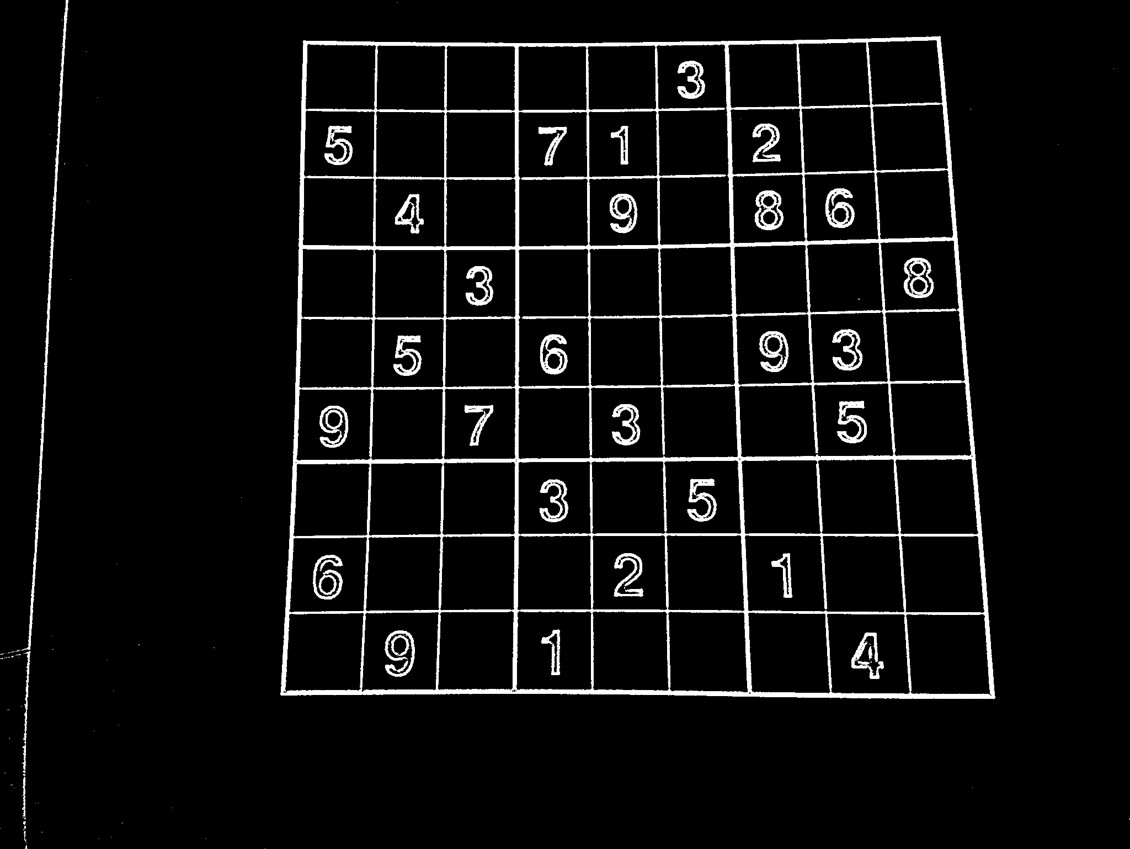
\includegraphics[scale=0.2]{../pictures/threshold.jpg}
 \caption{Exemple de grille "seuillée"}
 \end{figure}
 
Par cette transformation, on peut ensuite déterminer des équations de droites des contours extérieurs de la grille. Les coordonnées des intersections des droites seront celle des coins de la grille. \smallbreak On découpe alors la grille de la photographie initiale en supprimant les éventuels effets de perspective. 
 
\begin{figure}[!h]
 \center
 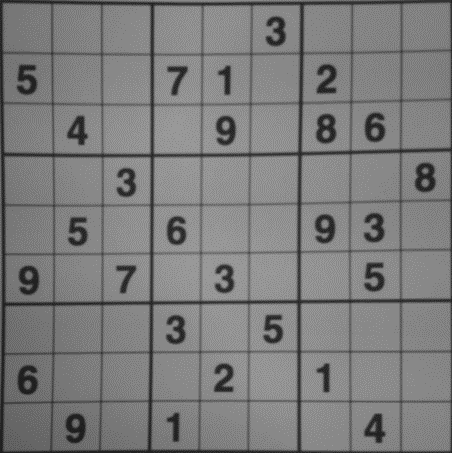
\includegraphics[scale=0.45]{../pictures/unperspectived.png}
 \caption{Exemple de grille découpée sans perspective}
\end{figure}
\newpage
On découpe chaque petite case de la grille comme ci-dessous :

\begin{figure}[!h]
 \center
 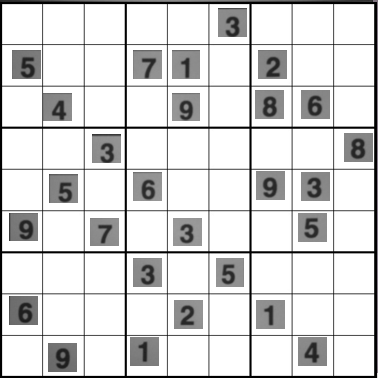
\includegraphics[scale=0.6]{../pictures/cutted.png}
 \caption{Exemple de grille où chaque chiffre a été découpé}
\end{figure}

On utilise ensuite un module de reconnaissance de digits pour détecter les chiffres et on obtient la grille suivante, prête à être résolue :

\begin{figure}[!h]
 \center
 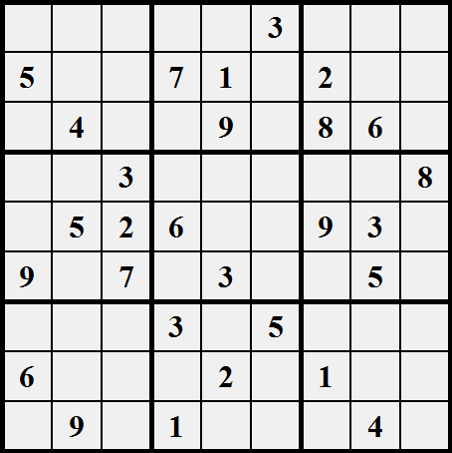
\includegraphics[scale=0.5]{../pictures/finished.png}
 \caption{Exemple de grille prête à être résolue}
\end{figure}
\newpage

\section{Résolution du sudoku}
	
	\section{Écriture et contrôle des moteurs}
	

\printbibliography
\nocite{*}
\appendix
\begin{changemargin}{-2cm}{-4cm}
\chapter{Fichier principal}
\label{main}
\inputminted[fontsize=\scriptsize, linenos=true]{Python}{../script/main.py}
\chapter{Script de résolution des sudokus}
\label{resolution}
\inputminted[fontsize=\scriptsize, linenos=true]{Python}{../script/resolution.py}
\chapter{Script de gestion de la caméra}
\label{camera}
\inputminted[fontsize=\scriptsize, linenos=true]{Python}{../script/camera.py}


\end{changemargin}
\end{document}
